% Print
\documentclass[headinclude=true]{scrartcl}

%Packages, die für die englische Sprache
\usepackage[utf8]{inputenc}
\usepackage[T1]{fontenc}
\usepackage{lmodern}
\usepackage[english]{babel}
\usepackage{csquotes}

%Packages für Graphik
\usepackage[]{graphicx}
\graphicspath{{figures/}}

%BibLaTex
\usepackage[backend=biber]{biblatex}
\addbibresource{literature/bibliography.bib} 

%Package, damit Bibtex-URL klappt
\usepackage[pdfusetitle]{hyperref}
\usepackage{url}

\usepackage[section]{placeins}

%Noch schönere Typographie
\usepackage{microtype}

%Euro
\usepackage{eurosym}

%Kästen
\usepackage{framed}

%Package für schöne Tabellen mit variabler Breite
%\usepackage{tabularx}
\usepackage{tabulary}
\usepackage{booktabs}

\usepackage{todonotes}

%%%%% BEGINN KOPF- UND FUẞZEILE %%%%%
%\usepackage[]{scrlayer-scrpage}
%\pagestyle{scrheadings}
%\ohead{
\includegraphics[height=1cm]{figures/MPM_Logo}}
%\chead{\headmark}
%\automark{section}
%\ihead{
\includegraphics[height=1cm]{figures/TU_Logo}}
%\ifoot{\csname @title\endcsname}\cfoot{\pagemark}
%\ofoot{\today}
%%%%% ENDE KOPF- UND FUẞZEILE %%%%%

\begin{document}

%%%%% BEGINN TITEL %%%%%
\title{Semester Task}
\subtitle{Systematic Product Development}
\author{Alexander Grahle \and Ludger Heide \and Dr. Tu-Anh Fay}
\titlehead{\centering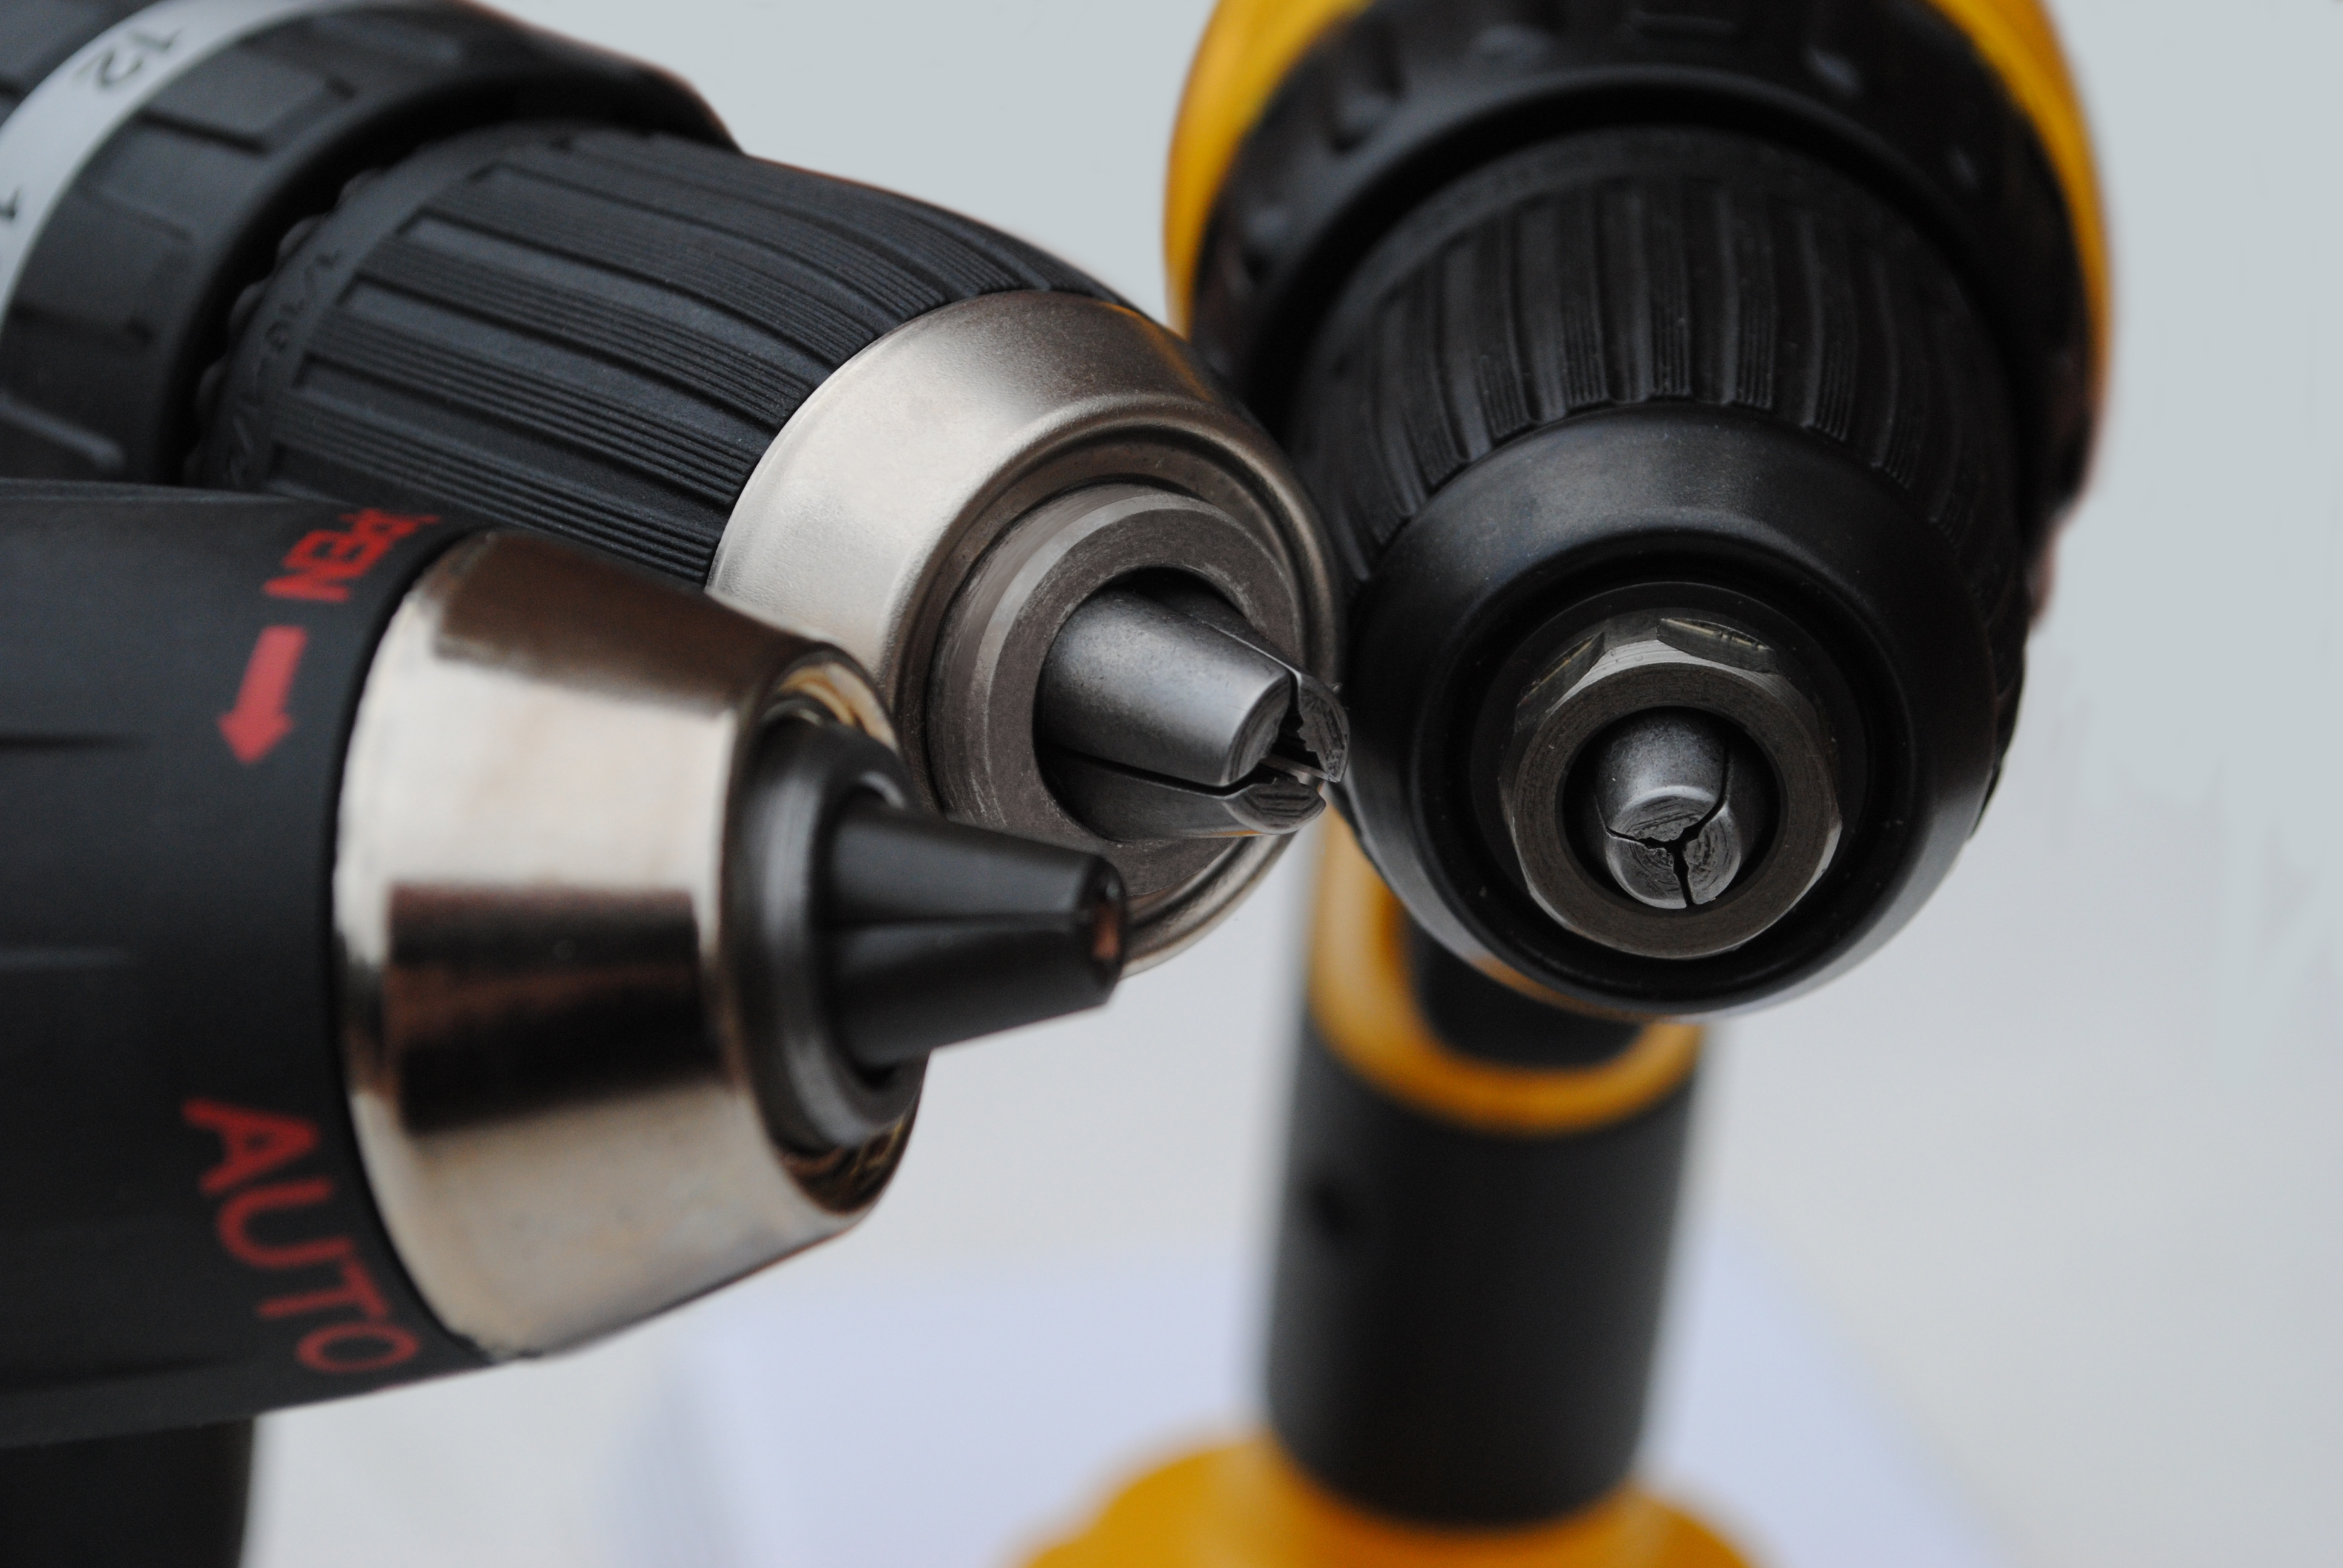
\includegraphics[width=\textwidth]{drills}}
\maketitle
\clearpage
%%%%% ENDE TITEL %%%%%

%%%%% BEGINN FRONT MATTER %%%%%
%\pagenumbering{roman}
\tableofcontents
%%%%% ENDE FRONT MATTER %%%%%


%%%%% BEGINN INHALT %%%%%
\clearpage
%\pagenumbering{arabic}
\section{About this document}

This document serves as a consolidated description of the things in the course ``Systematic Product Development'' (SPD) that are relevant to grading. It contains information on how grades are calculated as well as the official documentation of the group task. While we aim to keep the defintion of the task consistent throughout the semester, this is a ``living document'' into which the clarifications made in response to your questions will be incorporated. Its version history is maintained on GitHub\footnote{\url{https://github.com/mpm-tu-berlin/lehre-spd}}. 

\section{Grading}

\subsection{Exam Components}

The exam is composed of four different components. Three of these (presentation, 1\textsuperscript{st} and 2\textsuperscript{nd} project report) are conducted in groups, the final exam is conducted individually. The weighing of these components is shown in table \ref{tab:komponenten}.

\begin{table} \centering
 \caption{Point Distribution}
 \label{tab:komponenten}
 \begin{tabular}{lr}
  \toprule
  Component & Points \\ \midrule
  1\textsuperscript{st} submission of project report & 10 \\ 
  2\textsuperscript{nd} submission of project report & 25 \\ 
  Presentation of project results & 15 \\ 
  Digital examination & 50 \\ \midrule
  \textbf{Sum} & \textbf{100} \\ \bottomrule
 \end{tabular}
\end{table}

\subsubsection{Project Report}

The task for the project report is explained in detail in section \ref{chap:projektaufgabe}.

\subsubsection{Presentation of Project Results}

\todo[inline]{Presentation -- a little bit like in EnWiNaP, focusing on the unique features of each solution rather than each group showing the same thing. Perhaps each group focuses on one topic like cost, morphological box etc.?}

\subsubsection{Digital examination}

The final exam will be conducted online on ISIS as an individual task. It will consist both of multiple choice questions and freeform questions testing both straight-up reproduction of the course knowledge (for example ``fill in the blanks'') as well as application (for example ``identify problems and recommend solutions for a given analysis''). There will be XX\todo{What aids are allowed?} aids such as written notes allowed.

\subsection{Grading Scale}

The final grade is calculated as follows:

\begin{enumerate}
 \item The component percentages are rounded to full points. Example: Getting 84\% in a 10-point component leads to 8 points for this component.
 \item The points for each component are summed up.
 \item The final grade is calculated according to table \ref{tab:notenskala}
\end{enumerate}

Please note that if any part of the exam is failed due to scientific fraud (e.g. plagiarism), the whole module will be graded as ``failed'' and will need to be repeated.

\begin{table} \centering
 \caption{Grading Scale}
 \label{tab:notenskala}
 \begin{tabular}{rr}
  \toprule
  Points & Grade \\ \midrule
  $\geq$ 95 & 1,0 \\
  $\geq$ 90 & 1,3 \\
  $\geq$ 85 & 1,7 \\
  $\geq$ 80 & 2,0 \\
  $\geq$ 75 & 2,3 \\
  $\geq$ 70 & 2,7 \\
  $\geq$ 65 & 3,0 \\
  $\geq$ 60 & 3,3 \\
  $\geq$ 55 & 3,7 \\
  $\geq$ 50 & 4,0 \\
  $<$ 50 & 5,0 \\ \bottomrule
 \end{tabular}
\end{table}

\section{The Truly Cordless Drill}
\label{chap:projektaufgabe}

\begin{figure}[h!] \centering
 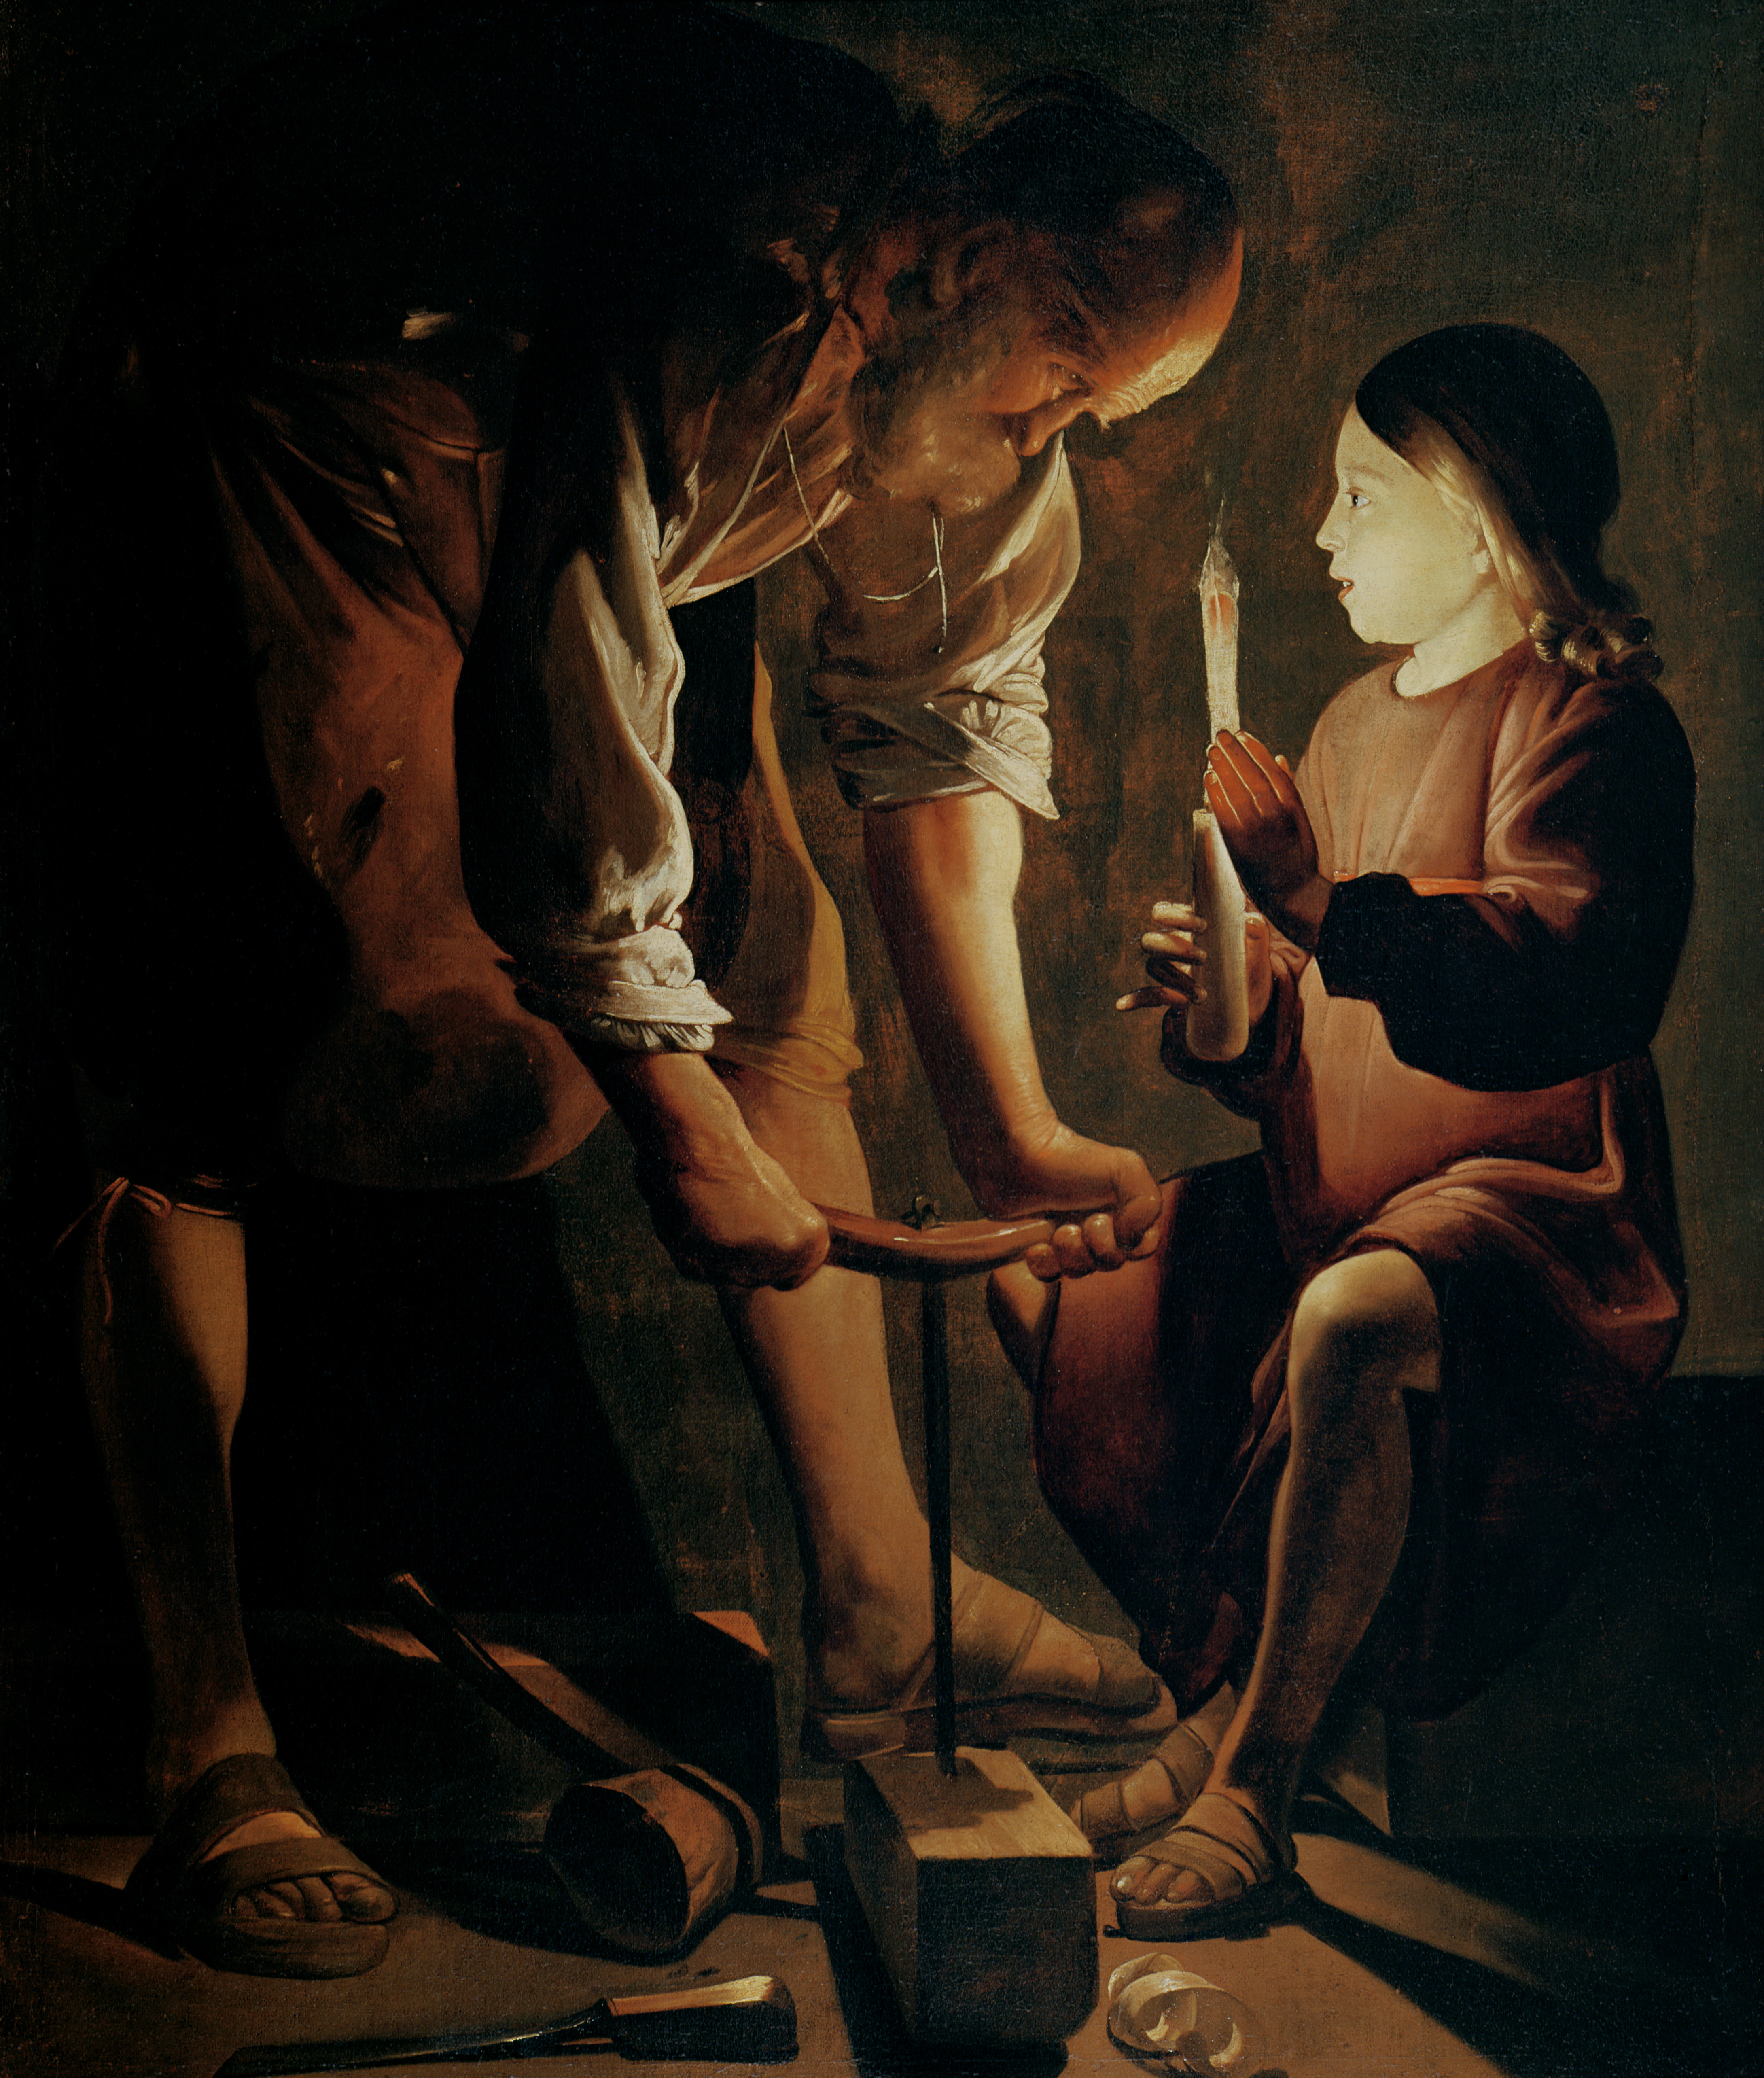
\includegraphics[width=0.5\linewidth]{La_Tour}
 \caption{Not an acceptabke solution: Manual operation without energy storage. Image: ``Saint Joseph charpentier'' by Georges de La Tour (1593–1652).}
\end{figure}


Your task for this semester will be to design a cordless drill. There is a twist though: It should work without utilitzing any electricity. By this we mean that it should still work if all physical laws governing the flow of electricity in (semi)conductors were not to exist. Electrical motors, batteries and capacitors are out, as are electric switches and silicon-based control systems.

Specifically, what we are asking you to design is a

\begin{itemize}
 \item Hand-holdable
 \item Rechargeable
\end{itemize}

device to produce

\begin{itemize}
 \item A peak torque $M_{max}$ of 50~Nm
 \item A no-load rotational speed $\eta_1$ of 1500~$\frac{1}{min}$
 \item With the ability to do useful work at intermediate speeds and torques
 \item As selected by the user's graduated power demand
 \item For 5 minutes of continuous operation at the maximum power point without recharging
 \item applied to an industry-standard $\frac{1}{4}$-inch hexagonal socket according to DIN~ISO~1173 form D. \cite{DDIN2009}.
\end{itemize}

\begin{figure} \centering
 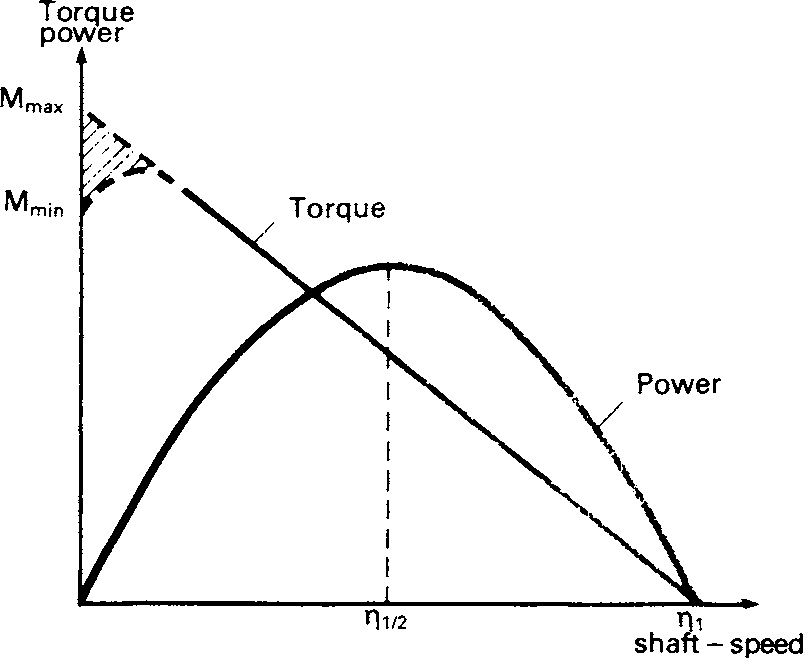
\includegraphics[width=0.5\linewidth]{speed-torque}
 \caption{Exemplary speed-torque curve. Yours may differ! Source: \cite{Barber1997}}
\end{figure}


You are allowed to use a two-speed geared design. This device must operate and recharge without using any electricity, but it could be manufactured by processes that require electricity (so you don't need to design a mechanical lathe as well).

\subsection{Tasks for the Project Report}

The project report shall be a report on the development of your solution to the semester task. It should be a well-written technical/scientific report that contains the subtasks shown below. We expect these subtasks to be linked together in a reasonable structure, as well as an introduction describing the problem and a conclusion. It should observe the rules of good scientific and engineering practice as well as the stylistic ``rules'' of good typography. It should not exceed XX\todo{Fill in pages for first submission} content pages\footnote{``Content pages'' refers to the page count excluding front and back matter, such as table of contents, bibliography etc.} for the 1\textsuperscript{st} submission and XX\todo{Fill in pages for the second submission} for the 2\textsuperscript{nd} submission. The 1\textsuperscript{st} submission should be submitted as a PDF file, the 2\textsuperscript{nd} submission should be submitted as a \texttt{.zip} archive containing the PDF report and the additional files.

\subsubsection{1\textsuperscript{st} submission}
The 1\textsuperscript{st} submission consists of the following subtasks:
\begin{itemize}
 \item One SWOT analysis for the team skills and one for the product idea developed in the first workshop.
 \item A list of rquirements according to Pahl/Beitz \cite{Pahl2007}, using the template given on ISIS.
 \item A functional structure with sub-functions and the derivation of working principles for these subfunctions.
 \item A morphological box showing all possible sub-solutions.
 \item The systematic derivation of at least three possible solution variants using a reduced morphological box.\footnote{Completing this task requires the application of selection and evaluation methods. This has been missed by some groups in the past.}
 \item Coherent explanation and sketches of these three solutions
 \item Applying a weighing and value scales to the evaluation criteria shown in section \ref{sec:evaluation}.
\end{itemize}

\subsubsection{2\textsuperscript{nd} submission}
The 2\textsuperscript{nd} submission consists of the following subtasks:
\begin{itemize}
 \item All content of the first submission, with revisions as per our corrections.
 \item A selection of a final concept using performance calculations and coherent assumptions.
 \item A detailed design of the final concept:
 \begin{itemize}
  \item A short functional description of the final concept with detailed pictures/drawings of the main functions.
  \item A calculation of the primary performance characteristics, describing the relevant mathematical formulas and showing the calculation of torque, no-load speed, power and energy.
  \item A risk assessment (FMEA).
  \item A parts list specifying the sourcing and cost of each part.
  \item A 3D CAD model in the STEP format.
  \item A plot showing the main dimensions of the final product.
  \item Manufacturing drawings (PDF) for the ``classical'' custom-made parts and STL files for the custom-made parts utilizing additive manufacturing.
 \end{itemize}

\end{itemize}

\subsection{Evaluation Criteria}
\label{sec:evaluation}

The following evaluation criteria listed in table \ref{tab:evaluation} should be used by you for selecting your final concept and will guide us in which design we wil (hopefully) attempt to actually build.

\begin{table}
\caption{Evaluation criteria}
\label{tab:evaluation}
 \begin{tabulary}{\linewidth}{lLll}
 \toprule
 Criterion & Description & Value & Remark \\ \midrule
 Peak torque & The peak torque available at the output shaft. & 50~Nm & Minimum value \\
 Peak speed & The no-load rotational speed of the output shaft. & 1500 $\frac{1}{min}$ & Minimum value \\
 Energy & The device shall operate for the given time at its maximum power. & 5 minutes & Target value \\
 Cost & The total price of the prototype not including final assembly labor. & 500 \euro & Target value \\
 Reliability & The number of charge and operation cycles without mainenance intervention. & 10 & Target value \\
 Control & The device shall be able to drive a wood screw into a pieces of soft and hard wood without damaging the workpiece or screw. & N/A & Target \\ \bottomrule
 
 
  
 \end{tabulary}
\end{table}






%%%%% ENDE INHALT %%%%%

%%%%% BEGINN BACK MATTER %%%%%

%%%%% Ende Back Matter %%%%%
\printbibliography

\appendix

\end{document}
